\documentclass[11pt]{article}

\usepackage{amsmath}
\usepackage{textcomp}
\usepackage{graphicx}     
\usepackage[top=0.8in, bottom=0.8in, left=0.8in, right=0.8in]{geometry}
% add other packages here

\usepackage[ruled,vlined]{algorithm2e}

% put your group number and names in the author field
\title{\bf Exercise 2: A Reactive Agent for the Pickup and Delivery Problem}
\author{Group \textnumero: 272257, 262609}

% the report should not be longer than 3 pages

\begin{document}
\maketitle

\section{Problem Representation}

\subsection{Representation Description}
% describe how you design the state representation, the possible actions, the reward table and the probability transition table

 	The problem studied in this report is the classical pickup and delivery problem. We try here specifically to implement one agent (which will be reffered to as \emph{the truck} or the agent interchangeably from now on). We try to implement the truck as a reactive agent. 
 	To properly explain the comportment of the agent, we need to clearly state what are : \emph{the states}, \emph{the actions}, \emph{the reward table}, and \emph{the probability transition table}.
 	\begin{itemize}
 		 \item[$\bullet$] \textbf{States}: The state represents the perception that the agent has of it's environment. Once the agent finishes an action (see definition of actions), it observes two things: the city it arrived in and the task (or absence thereof) it may accept. In our implementation, the states are represented in memory by two attributes: the city the agent is currently in and the city the task points to. Note that \textbf{the absence of task is represented by a contract from the current city to itself}.
 		 
 		 \item[$\bullet$] \textbf{Actions}: An action is defined as the movement of the agent from a city to another. Note that actions can describe the movement of the agent from any city to any other one \textbf{even if the two cities are not connected directly}.
 		 
 		 \item[$\bullet$] \textbf{Reward table}: The reward table is a $\# States\times\# Actions$ table in which each cell gives us the reward given to the agent if it is in a given state and chooses a given action. For two cities $i$ and $j$, we are given the average reward of a contract from $i$ to $j$, which will be denoted $r(i,j)$ and thus each cell will either contain zero, if the departure city and arrival city of the state and the action do not coincide, either contain $r(i,j)$ if they do.
 		 
 		 \item[$\bullet$] \textbf{Probability transition table}: The probability transition table is a $\# States\times\# Actions\times\# States$ table that gives us the probability of being in the state $s'$ if the action $a$ is performed in the state $s$. Note that if the city of departure of $a$ is not the current city of $s$ or the city of arrival of $a$ is not the current city of $s'$, then this probability is zero. Otherwise, we note that, since the city of the state of arrival is a deterministic variable when given a state and an action, we see that the probability is only determined by the probability of the presence of a contract from the city of $s'$, $i$, to the city of arrival of the contract given in $s'$, $j$. These probabilities are a given datum of the problem, and will be denoted $p(i,j)$.
	\end{itemize}
 		 
\subsection{Implementation Details}.
% describe the implementation details of the representations above and the implementation details of the reinforcement learning algorithm you implemented


In this implementation, we implement the actions as the class \emph{ActionMDP}, which comprises of two attributes: the first being \emph{City startCity} that represents the city the truck is currently in and an other \emph{City endCity} that represents the city will be in if the truck chooses the given action.

We implement the states as the class \emph{StateMDP}, which comprises of two attributes: the first being \emph{City city} that represents the city the agent is currently in and the second being \emph{City task} that represents the arrival city of the current task.

We implement the reward table as a method of the \emph{Reactive} class, \emph{rewardFunction(StateMDP startState, ActionMDP action)}. The output of this function for the a given state $s$ and an action $a$ is: 
 	\begin{align*}
 		rewardFunction(s,a)= 
 			\begin{cases}
 				0 & \mathrm{if}\ a.startCity\neq state.city,\\
 				r(s.city,a.endCity) & \mathrm{otherwise}
			\end{cases}
	\end{align*}
where $r(s.city,a.endCity)$  is given above.
 
We implement the probability transition table as a method of the \emph{Reactive} class, \emph{transitionProbabilities(StateMDP startState, ActionMDP action, StateMDP endState)}, which for given states $s,s'$ and an action $a$ gives us the following output:
	\begin{align*}
		transitionProbabilities(s,a,s')=
			\begin{cases}
				0 & \mathrm{if}\ a.startCity\neq s.city\ \mathrm{or}\ a.endCity\neq s'.city,\\
				p(s'.city,s'.task) & \mathrm{otherwise}
			\end{cases}
	\end{align*}
where $p(s'.city,s'.task)$ is defined above.
At a given state $s$, the action performed by the agent is given by the formula $$\pi(s)=\mathrm{argmax}_a\left\{rewardFunction(s,a)+\gamma\sum\limits_{s'\in S}transitionProbabilities(s,a,s')V(s')\right\}$$ where $S$ is the set of states, $\gamma$ is the discount factor, which is also a given datum of the proble, and $V(s)$ is the rewards that can be reached from the state $s$ using an optimal choice of actions, this is implemented as the \emph{policy} method of the \emph{Reactive} class. Note that the values $V(s)$ are thus given recursively by $$V(s) = \mathrm{max}_a\left\{rewardFunction(s,a)+\gamma\sum\limits_{s'\in S}transitionProbabilities(s,a,s')V(s')\right\}.$$ We use algorithm seen in class to approximate those values since this is actually a \textbf{Markov decision process} as the state transitions are not deterministic but we can analyze the current state with certainty:
	\begin{algorithm}[H]
		\SetAlgoLined
		%\Kwresult{A set of values V(s)}
	 	initialization: Set $V(s)$ arbitrary and $\infty \rightarrow V_{prev}(s)$ .\\	
	 	\While{$\mathrm{max}_s|V(s)-V_{prev}(s)| > \frac{0.01*(1-\gamma)}{2\gamma}$}{
	 		\For{$s\in S$}{
				$V(s) \rightarrow V_{prev}(s)$ \\
	 			\For{$a\in A$}{
	 				$Q(s,a) \leftarrow rewardFunction(s,a)+\gamma\sum_{s'\in S}transitionProbabilities(s,a,s')V(s')$
				}
				$V(s) \leftarrow \max_aQ(s,a)$
			}
		}
		\caption{Solving the MDP}
	\end{algorithm}
where $A$ is the set of actions. Note that this algorithms terminates since the set of rewards is finite and thus bounded. Also note that the number in the while condition is here to assure that when the algorithm terminates we have $\mathrm{max}_s|V(s)-V^*(s)| < \epsilon = 0.01$, where $V^*(s)$ is the \emph{true value of the state $s$}, the latter being the value we want to approximate.

\section{Results}
% in this section, you describe several results from the experiments with your reactive agent


\begin{figure}[h!]
	\centering
	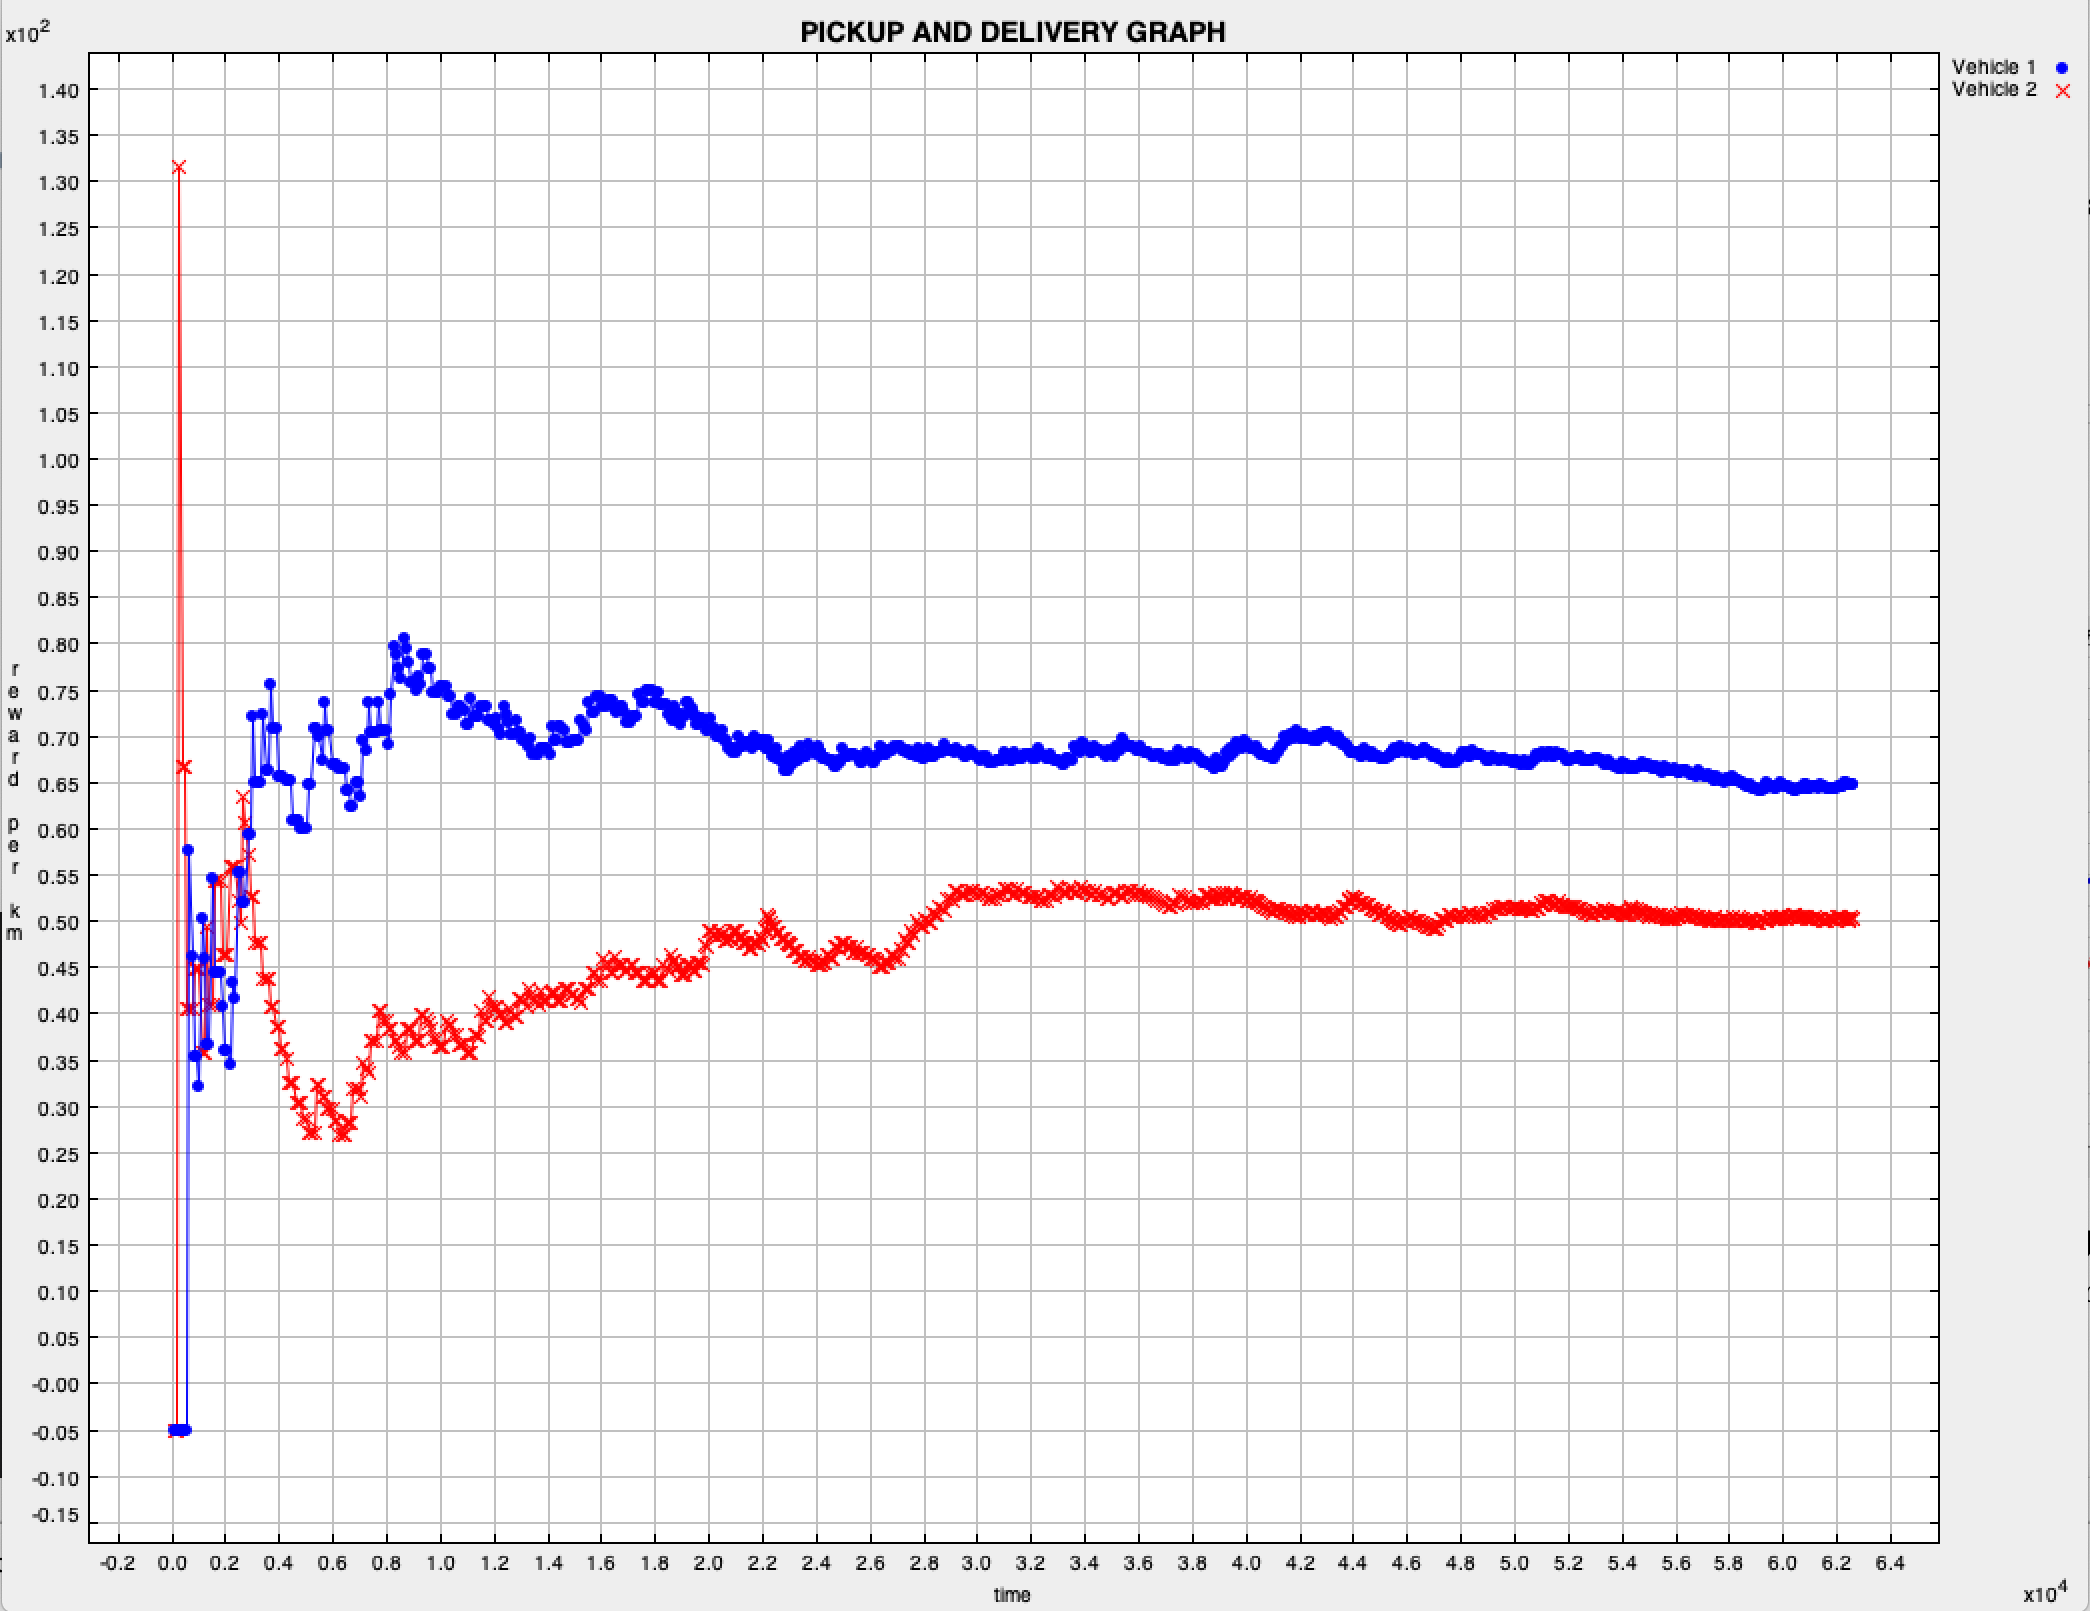
\includegraphics[width=0.4\textwidth]{figures/random_vs_mdp.png}
	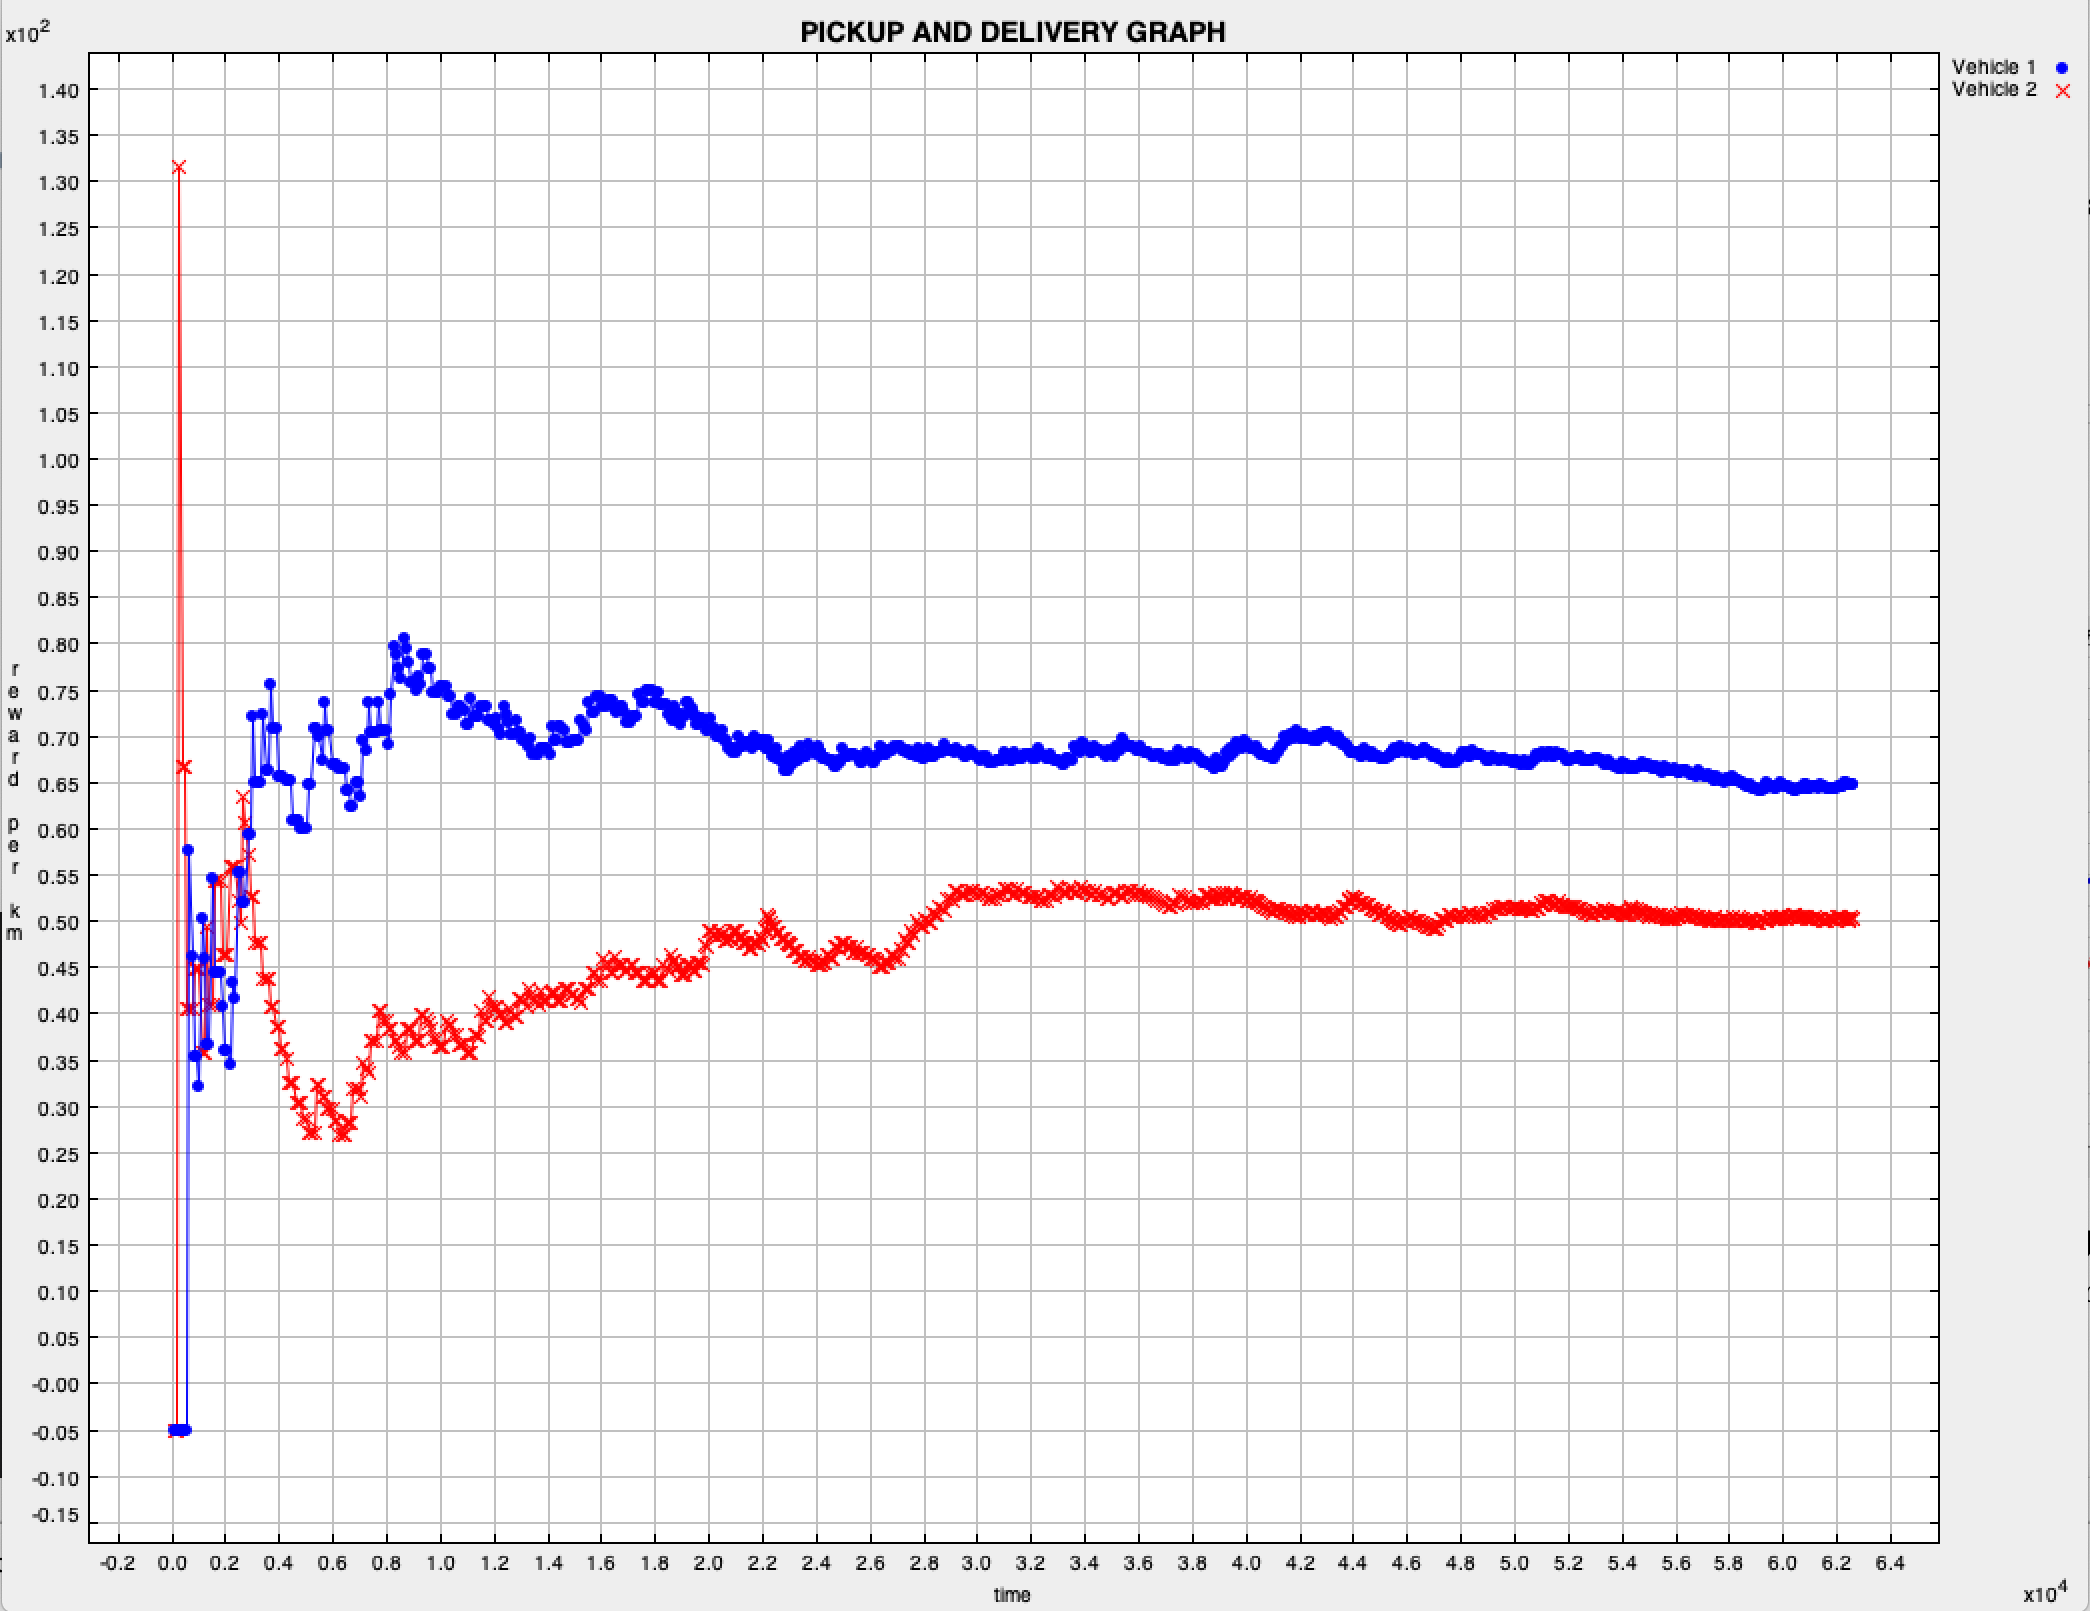
\includegraphics[width=0.4\textwidth]{figures/random_vs_mdp.png}
	\caption{\textbf{Left :} evolution over time of the average reward per kilometer for a reactive MDP agent (in blue, with a discount factor of $0.85$) and a dummy agent (that takes random decisions, in red). \textbf{Right :} Similar plot for the evolution of rabbit (red) and grass (green) population equilibriums as the grass growth rate changes.}
\end{figure}

\subsection{Experiment 1: Comparisons with dummy agents}
% you compare the results of your agent with two dummy agents: the random agent that was already given in the starter files and another dummy agent that you define and create. You should report the results from the simulations using the topologies given in the starter files and optionally, additional topologies that you create.
We compare one of our \emph{MDP} reactive agents (with a discount factor $\gamma = 0.85$) to a randomly action agent shows a clear performance difference, the topology is a model of France's road network.
% you describe how you perform the experiment and you describe the dummy agent you created (you also need to specify the configuration used for the experiment)

\subsubsection{Observations}
% elaborate on the observed results

 This is shown on Figure 1, left. But our algorithm maximizes the average reward per action not by kilometer, the experiment also clearly shows shows improvement by this metric : one a $250$ actions sample we have : 
 \begin{align*}
	 \textit{A total profit of $9926295$ (average / action : $39705.180$)} && \textit{for the reactive agent} \\
	 \textit{A total profit of $7987058$ (average / action : $31948.232$)} && \textit{for the dummy agent} 
 \end{align*}
 Our system is showing a $24,27\%$ improvement compared to the dummy base case.
 
 \subsubsection{Setting}
  

\subsection{Experiment 2: Discount factor}
% the purpose of this experiment is to understand how the discount factor influences the result

\subsubsection{Setting}
% you describe how you perform the experiment (you also need to specify the configuration used for the experiment)

\subsubsection{Observations}
% you describe the experimental results and the conclusions you inferred from these results

\end{document}